\section{Verschiedene Versionen der Anzeige}
\setauthor{Oliver Sugic}
Für die graphische Oberfläche wurden verschiedene Ideen und Konzepte ausprobiert, um die Benutzbarkeit für die Lernenden und Lehrenden zu optimieren.
Im Laufe des Kapitels wird erläutert, welche Versionen der Anzeige es gab und welche Versionen sich als sinnvoll erwiesen haben.

\subsection{Version 1: Visualisierung mit Karten}
\setauthor{Oliver Sugic}
Am Anfang wurden Überlegungen angestellt, wie man die Lernenden als auch die Lehrenden am besten in nicht vertrautes Gebiet führen kann.
Da die meisten Person mit Kartenservices, wie beispielsweise Google Maps oder ähnlichen Dienstleistungen, vertraut sind, wurde eine Karte implementiert.
Es gibt viele verschiedene Anbieter von Kartenservices, die in Betracht gezogen wurde. 
Da Google Maps eines der bekanntesten Anbieter, wurde die die Google Maps Api gesetzt. 
Doch im Laufe der Recherche ist klar geworden, dass die Google Maps Api nicht die beste Lösung für dieses Projekt ist  aus folgenden Gründen
\begin{itemize}
    \item Die Google Maps Api läuft über die Google Cloud und ist daher kostenpflichtig
    \item Google Maps Api ist nicht open-source
    \item Google Maps Api ist nicht einfach zu anzupassen an die Bedürfnisse des Projektes 
\end{itemize}
%\cite{}

Auf der Suche nach weiteren Alternativen, verwies mich Herr Pavelescu auf die Open-Source Kartenlösung Leaflet.
Leaflet ist eine JavaScript Libary, die es ermöglicht, Karten in Webanwendungen zu integrieren. 
\cite{Agafonkin}

\pagebreak

\begin{lstlisting}[numbers=left]
    <style>
    #map { height: 1000px; }
    </style>
    </head>
    <body>
     <link rel="stylesheet" href="https://unpkg.com/leaflet@1.9.3/dist/leaflet.css"
         integrity="sha256-kLaT2GOSpHechhsozzB+flnD+zUyjE2LlfWPgU04xyI="
         crossorigin=""/>
    
     <script src="https://unpkg.com/leaflet@1.9.3/dist/leaflet.js"
         integrity="sha256-WBkoXOwTeyKclOHuWtc+i2uENFpDZ9YPdf5Hf+D7ewM="
         crossorigin=""></script>
    
     <div id="map"></div>
      <script>
    var map = L.map('map').setView([48.2684159, 14.2517532], 20);
    L.tileLayer('https://tile.openstreetmap.org/{z}/{x}/{y}.png', {
        maxZoom: 19,
        attribution: '&copy; <a href="http://www.openstreetmap.org/copyright">OpenStreetMap</a>'
    }).addTo(map);
    </script> 
\end{lstlisting}

\begin{figure}[h t]
\centering
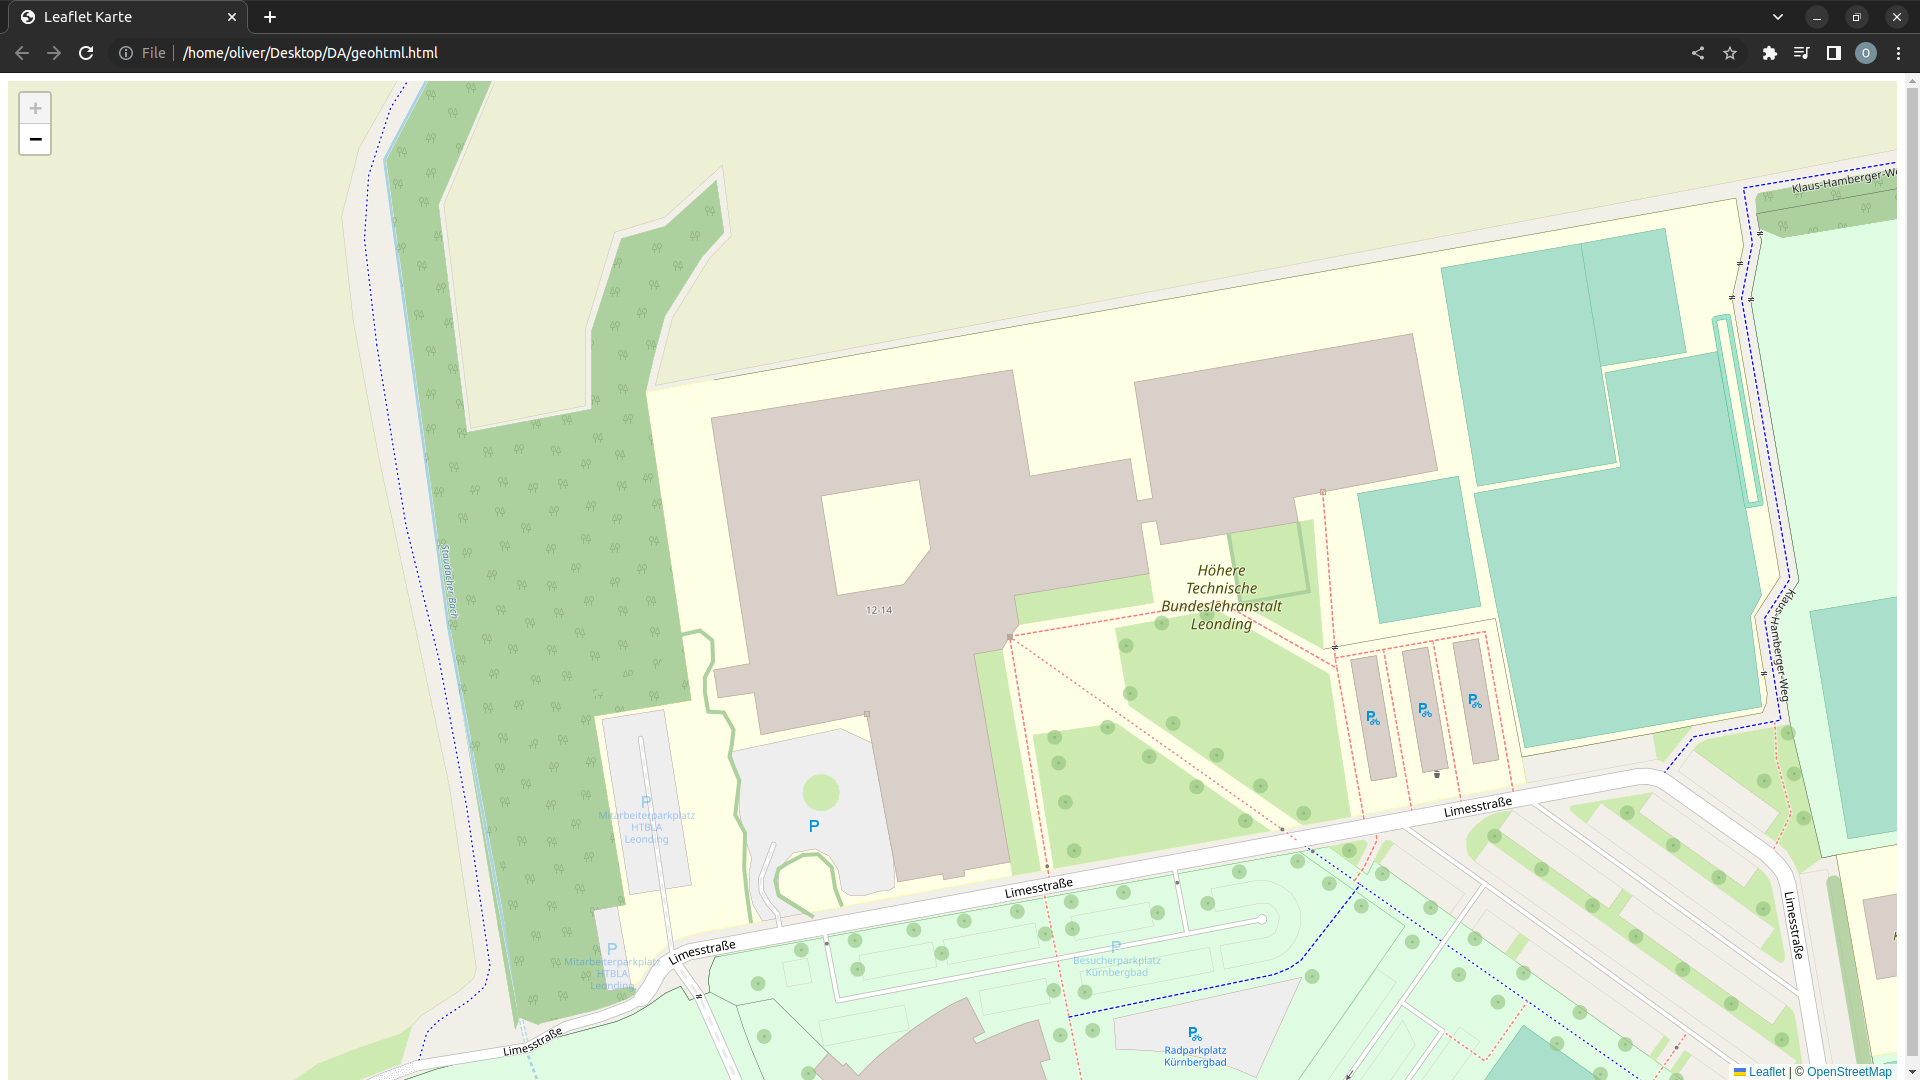
\includegraphics[scale=0.2]{pics/leafletmap.png}
\caption{Ergebnis der Implementierung mit Leaflet}
\end{figure}



\begin{spacing}{1}
\subsection{Version 2: Leaflet Karte mit Routing}
\setauthor{Oliver Sugic}
\end{spacing}

\begin{spacing}{1}
\subsection{Version 3: Angular Geoloaction API}
\setauthor{Oliver Sugic}
\end{spacing}

\begin{spacing}{1}
\section{Aktuelle Komponenten}
\setauthor{Oliver Sugic}
\end{spacing}

\begin{spacing}{1}
\subsection{Angular Frontend}
\setauthor{Oliver Sugic}
\end{spacing}

\begin{spacing}{1}
\section{Quarkus Backend }
\setauthor{Oliver Sugic}
\end{spacing}

\begin{spacing}{1}
\section{Keycloak}
\setauthor{Oliver Sugic}
\end{spacing}

\begin{spacing}{1}
\section{Mögliche zukünftige Erweiterungen}
\setauthor{Oliver Sugic}
\end{spacing}


